\section{Inledning}

\subsection{Bakgrund}
På vissa av Chalmers och Göteborgs Universitets program så är den första programmeringskursen i Haskell \citep{haskell98} och för en del av de nya eleverna är inlärningströskeln relativt hög. Vi tror att ett interaktivt webbverktyg skulle kunna sänka den här tröskeln och underlätta undervisningen. Ett webbverktyg medför även att man slipper installera och lära sig extra verktyg så som Glasgow Haskell Compiler (GHC) \citep{ghc}. Webbens stöd för interaktivitet gör det möjligt att snabbt visa funktionsdeklarationerna för de inbyggda funktionerna och att enkelt evaluera funktionerna och testa sig fram till olika resultat. 

En stor fördel med att ha tolken på webben är att det enda som behövs för att använda den är en javascriptkompatibel webbläsare, något som följer med i princip i alla moderna operativsystem.

Det är även så att många programmerare inte kommer i kontakt med funktionell programmering  och med hjälp utav ett interaktivt webbverktyg som är enkelt för användaren att använda så är våran förhoppning att fler människor ska komma i kontakt med funktionell programmering, och i synnerhet Haskell. Då flera moderna objektorienterade programmeringsspråk börjar ta begrepp och funktionalitet ifrån funktionella programmeringsspråk så är det extra viktigt att programmerare kommer i kontakt med funktionell programering. Ett exempel på detta är C\# som i senare versioner har fått stöd för bland annat lambdafunktioner \citep{csharp}. 


% TODO teori eller bakgrund?
Haskell är ett starkt statiskt typcheckat och funktionellt programeringsspråk med icke-strikt semantik. 
Att språket är funktionellt innebär bland annat att funktioner är \emph{first-class citizens} och kan därmed användas som parametrar och retuneras från andra funktioner precis som vilken annan typ som helst.

% TODO teori eller bakkgrund?
Icke strikt semantik, även kallat \emph{lazy evaluation}, innebär mer konkret att evalueringen av ett uttryck inte kommer utföras förrän resultatet av uttrycket behövs.
Lazy evaluation gör att programmeraren inte behöver bry sig om exekveringsordningen av ett program. Detta ger prestandaförbättringar eftersom ett uttryck inte evalueras alls om det inte behövs \citep{hudak89}.
Lazy evaluation gör det också möjligt att använda sig utav oändliga datastrukturer, till exempel oändliga listor. Språket blir därmed mer uttrycksfullt. 

Funktionella programmeringsspråk såsom Haskell anses också vara det naturliga steget att ta när man vill nå en högre abstraktionsnivå än den som imperativa programmeringsspråk tillåter.
Detta för att funktionella programmeringsspråk tillåter programmeraren att skriva program som är mer modulära, lättare att dela upp i separata delar, än imperativa programmeringsspråk. Den ökade modulariteten beror på att de stödjer tekniker såsom lazy evaluation och higher order functions.
Detta bidrar i sin tur yill att program skrivna i Haskell är generellt sätt kortare än ett program skrivet i ett imperativt programmeringsspråk. Detta gör att programmeraren blir mer produktiv i ett funktionellt programmeringsspråk kontra ett imperativt \citep{why}.

Med ovan nämnda resonemang ser vi det som ovärderligt för programmerare att komma i kontakt och ta del utav funktionell programmering. 
Vår förhoppning är att våran Haskelltolk i Javascript ska vara en inkörsport för programmerare till funktionell programmering.

\subsection{Syfte}
Syftet är en implementera en fungerande implementation av en haskkeltolk i Javascript. Den ska kunna tolka en delmängd utav Haskell-specifikationen så att den kan användas för att göra exempelvis interaktiva tutorials för nybörjare.
Meningen är att dessa ska kunna köras i en vanlig webbläsare utan att ladda ner en haskellkompilator, till exempel GHC, eller behöva lära sig krångliga kommandon.

\subsection{Problem} 

\subsection{Metod} 
Det normala tillvägagångssättet när man skriver en tolk är att man först
skapar en parser för den aktuella syntaxen, sedan en typcheckare med 
hjälp av de för språket definierade typereglerna och sist en interpreter
som tolkar språket utefter dess specifikation.

Vi hade tänkt följa den här planen genom varje milstolpe genom att utöka parsern, typecheckaren och interpretern med ny funktionalitet.

Ett lämpligt delmål är att först göra en enkel implementation utav lambda calculus då mer avancerade funktionella programspråksegenskaper kan implementeras som detta \citep{jones87}

 Parsern implementeras med hjälp av ett parser combinator bibliotek kallat \emph{JSParse} \citep{jsparse}. Detta ger oss möjlighet att implementera den del av Haskells syntax som inte är context free relativt enkelt.

Vi kommer även att använda det biblioteket för att bygga ett eget syntaxträd som skickas vidare till typcheckaren och interpretern. I typcheckaren dekoreras syntaxträdet med typinformation.

Vi kommer att integrera JQuery \citep{jquery} för att få unisont stöd över samtliga webbläsare utan att behöva tänka på det. JQuery kommer också hjälpa oss med att få till ett enkelt och stilrent interaktivt gränssnitt.

\subsubsection{Avgränsningar}
Att tolka Haskell i Javascript är inget trivialt projekt. Därför kommer inte hela Haskell att implementeras. 
Endast en delmängd av Haskell98 specifikationen kommer att implementeras. De delar som prioriterades är
        \begin{enumerate}
            \item{lambda-funktioner, namngivna funktioner}
            \item{typer, generella typer, algebraiska datatyper}
            \item{typklasser}
            \item{pattern matching}
            \item{Guards}
            \end{enumerate}
Med dessa delar implementerade kan de flesta enklare haskellprogram köras och borde vara tillräckligt för det stora flertalet nybörjare. Man ska komma ihåg att detta projekt inte kommer resultera i något som ska ses som ett komplement till vanliga haskellkompilatorer, såsom GHC och Hugs, utan en snabbare inkörsport för att lära sig Haskell. Därför anser vi att detta är en bra kompromiss för som gagnar Haskellcommunityn mest. % :D :D: D

\begin{figure}
    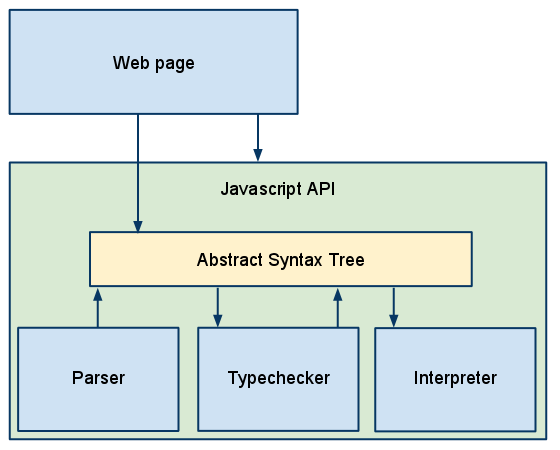
\includegraphics{image1.png}
    \caption{Överblick över tolkens struktur och interaktion}
\end{figure}
